\subsection*{RQ2: Coding Agent Harness Usage (@Mira and team)}
\emph{Which coding agent harnesses do hyperactive developers use, and for which tasks?}


% Note, use agent harness (or just harness) to clarify we mean the software around the agent, not individual agent instances or the model used by the agent. See fabis original comment below.
% (Fabi): should we consistently refer to it as "agent harnesses" to make it obvious that we're talking about different types of agents () as opposed to just multiple agent instances or sub-agents (i.e. multiple terminals all running an instance of Claude Code)?


% \begin{itemize}
%   \item Motivation; why is this RQ important?
%   \item Metrics: agent signal rate per month, agent diversity per developer, agent-switch events.
%   \item Expected analyses: \texttt{detect-agents.py}, \texttt{plot-agent-commit-coevolution.py}.
%   \item Hypothesis: agent concentration increases over time; \texttt{claude\_code} dominates late in the window; developers switch primary agents.
%   \item
% \end{itemize}


To study coding agent harness usage, we analyze repository activity at the commit level and infer which harness was used for each commit. We define a \emph{coding agent harness} as the software interface through which a developer interacts with an LLM-based coding agent, such as Claude Code, OpenAI Codex, Cursor, or Pi. We define an \emph{agent signal} as observable evidence linking a commit to a specific harness. A commit is assigned to a harness if at least one of the following conditions holds:

\begin{itemize}
\item the commit author name or co-author trailers mention a known harness;
\item the commit modifies harness-specific configuration or metadata files;
\item the commit message contains explicit harness identifiers.
\end{itemize}

% documentation on commit trailers:
% amp has them, yet we basically never see them (95 commits total)
% https://ampcode.com/manual#:~:text=Enable%20adding%20Amp%2DThread%20trailer%20in%20git%20commits%2E%20When%20disabled%2C%20commits%20made%20by%20the%20agent%20will%20not%20include%20the%20Amp%2DThread%3A%20%3Cthread%2Durl%3E%20trailer

A commit without such evidence is classified as \emph{unattributed}. Some harnesses append attribution metadata by default (e.g., Claude Code or Codex co-author trailers), while others leave little or no commit-level trace. Consequently, the absence of a detectable signal does not imply the absence of agent usage. Since this research question requires a harness assignment for all commits, unattributed commits are assigned using a fallback strategy. For each repository and developer, we determine the dominant harness among attributed commits within the surrounding development period and assign unattributed commits to that harness. We evaluate the sensitivity of this approximation with manual validation. We compute the following metrics:

\begin{itemize}
\item \textbf{Agent signal rate}: proportion of commits per month containing detectable harness signals.
\item \textbf{Harness frequency}: number and proportion of commits attributed to each harness.
\item \textbf{Harness diversity}: number of distinct harnesses used by a developer within a time window.
\item \textbf{Harness-switch events}: changes in the dominant harness used by a developer or repository over time.
\item \textbf{Cross-repository reuse}: extent to which the same harnesses appear across multiple repositories owned by the same developer.
\end{itemize}

\paragraph{Task classification.}
To analyze which tasks developers use agents for, we categorize commits using the Conventional Commits specification\footnote{\url{https://www.conventionalcommits.org/en/v1.0.0/}}. Prior work by Robbes et al.~\cite{Robbes2026} found that agent-assisted commits frequently follow these conventions, making them suitable for commit-level task categorization. For each harness, we analyze the distribution of commit categories (e.g., \texttt{feat}, \texttt{fix}, \texttt{refactor}, \texttt{docs}) to identify differences in harness usage across development tasks.


\begin{figure*}[t]
\centering
\begin{subfigure}{0.47\textwidth}
  
\includegraphics[width=\linewidth]{figures/rq2/rq2-agent-use-mavam.pdf}
  \caption{mavam}
  \label{fig:rq2-mavam}
\end{subfigure}\hfill
\begin{subfigure}{0.47\textwidth}
  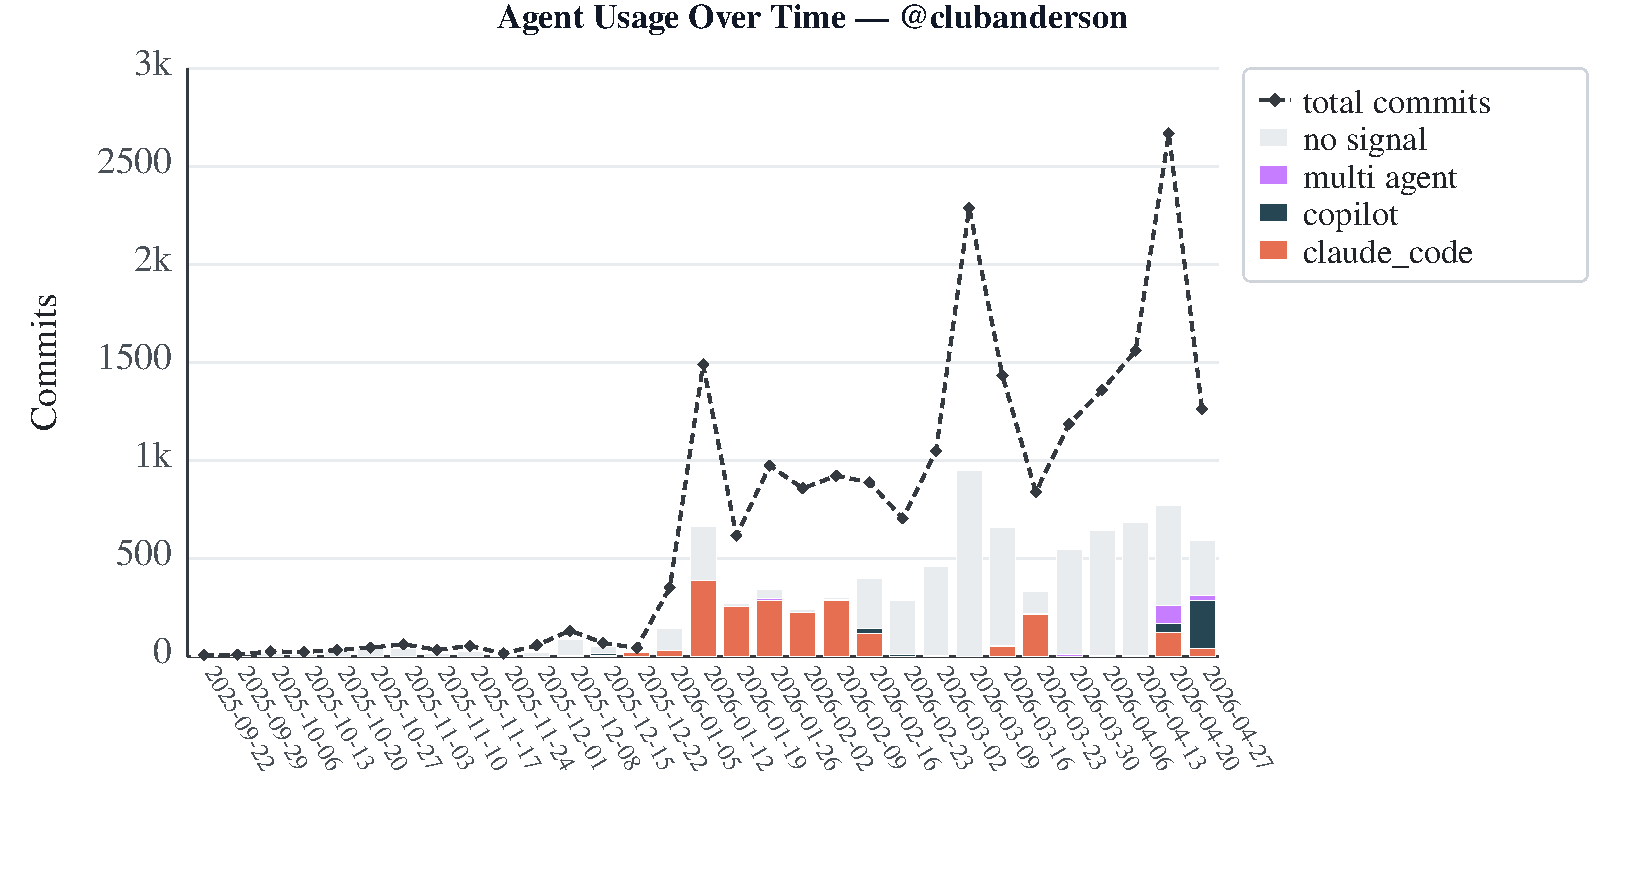
\includegraphics[width=\linewidth]{figures/rq2/rq2-agent-use-clubanderson.pdf}
  \caption{clubanderson}
  \label{fig:rq2-clubanderson}
\end{subfigure}

\begin{subfigure}{0.47\textwidth}
  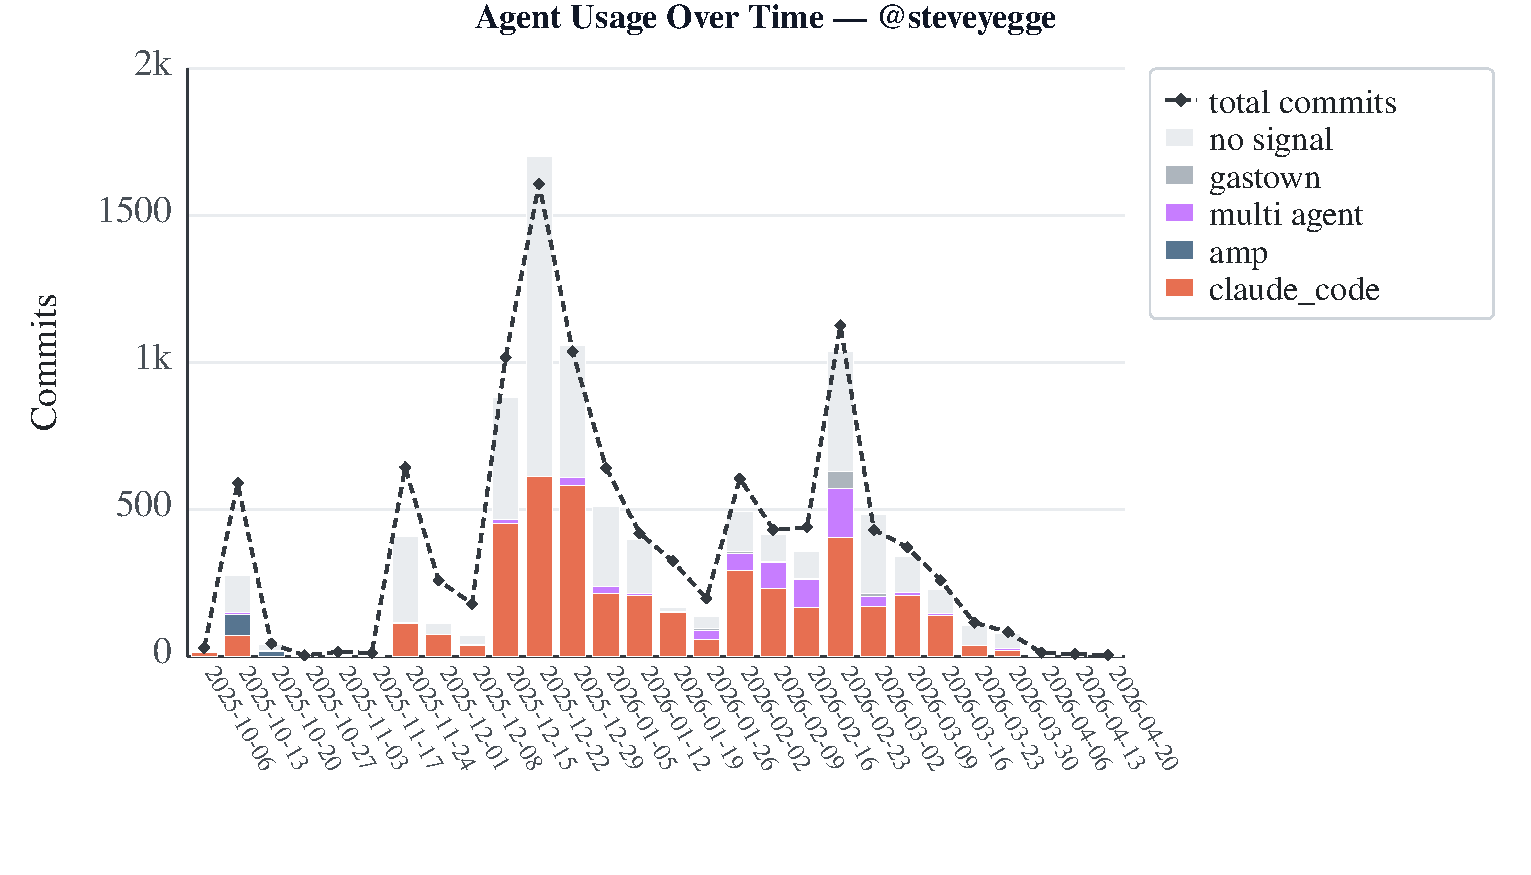
\includegraphics[width=\linewidth]{figures/rq2/rq2-agent-use-steveyegge.pdf}
  \caption{steveyegge}
  \label{fig:rq2-steveyegge}
\end{subfigure}\hfill
\begin{subfigure}{0.47\textwidth}
  
\includegraphics[width=\linewidth]{figures/rq2/rq2-agent-use-teamchong.pdf}
  \caption{teamchong}
  \label{fig:rq2-teamchong}
\end{subfigure}

\begin{subfigure}{0.47\textwidth}
  
\includegraphics[width=\linewidth]{figures/rq2/rq2-agent-use-steipete.pdf}
  \caption{steipete}
  \label{fig:rq2-steipete}
\end{subfigure}\hfill
\begin{subfigure}{0.47\textwidth}
  
\includegraphics[width=\linewidth]{figures/rq2/rq2-agent-use-ruvnet.pdf}
  \caption{ruvnet}
  \label{fig:rq2-ruvnet}
\end{subfigure}

\begin{subfigure}{0.47\textwidth}
  
\includegraphics[width=\linewidth]{figures/rq2/rq2-agent-use-obra.pdf}
  \caption{obra}
  \label{fig:rq2-obra}
\end{subfigure}\hfill
\begin{subfigure}{0.47\textwidth}
  
\includegraphics[width=\linewidth]{figures/rq2/rq2-agent-use-Dicklesworthstone.pdf}
  \caption{Dicklesworthstone}
  \label{fig:rq2-Dicklesworthstone}
\end{subfigure}

\begin{subfigure}{0.47\textwidth}
  
\includegraphics[width=\linewidth]{figures/rq2/rq2-agent-use-philipp-spiess.pdf}
  \caption{philipp-spiess}
  \label{fig:rq2-philipp-spiess}
\end{subfigure}\hfill
\begin{subfigure}{0.47\textwidth}
  \caption*{}
\end{subfigure}
\caption{Agent usage over time for each developer. Stacked bars show the distribution of detected agent harnesses per week. Solid and dashed lines show total and sampled commit counts respectively.}
\label{fig:rq2-agent-use}
\end{figure*}

\begin{figure*}[t]
\centering
\begin{subfigure}{0.47\textwidth}
  
\includegraphics[width=\linewidth]{figures/rq2/commit-types-agent-codex.pdf}
  \caption{Codex}
  \label{fig:rq2-codex}
\end{subfigure}\hfill
\begin{subfigure}{0.23\textwidth}
  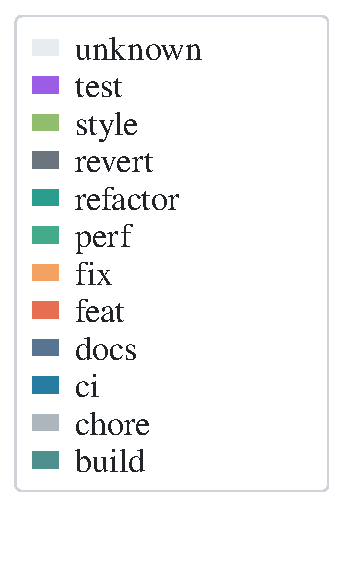
\includegraphics[width=\linewidth]{figures/rq2/commit-types-legend.pdf}
  \caption{Legend}
  \label{fig:rq2-commit-types-legend}
\end{subfigure}

\begin{subfigure}{0.47\textwidth}
  
\includegraphics[width=\linewidth]{figures/rq2/commit-types-agent-copilot.pdf}
  \caption{Copilot}
  \label{fig:rq2-copilot}
\end{subfigure}\hfill
\begin{subfigure}{0.47\textwidth}
  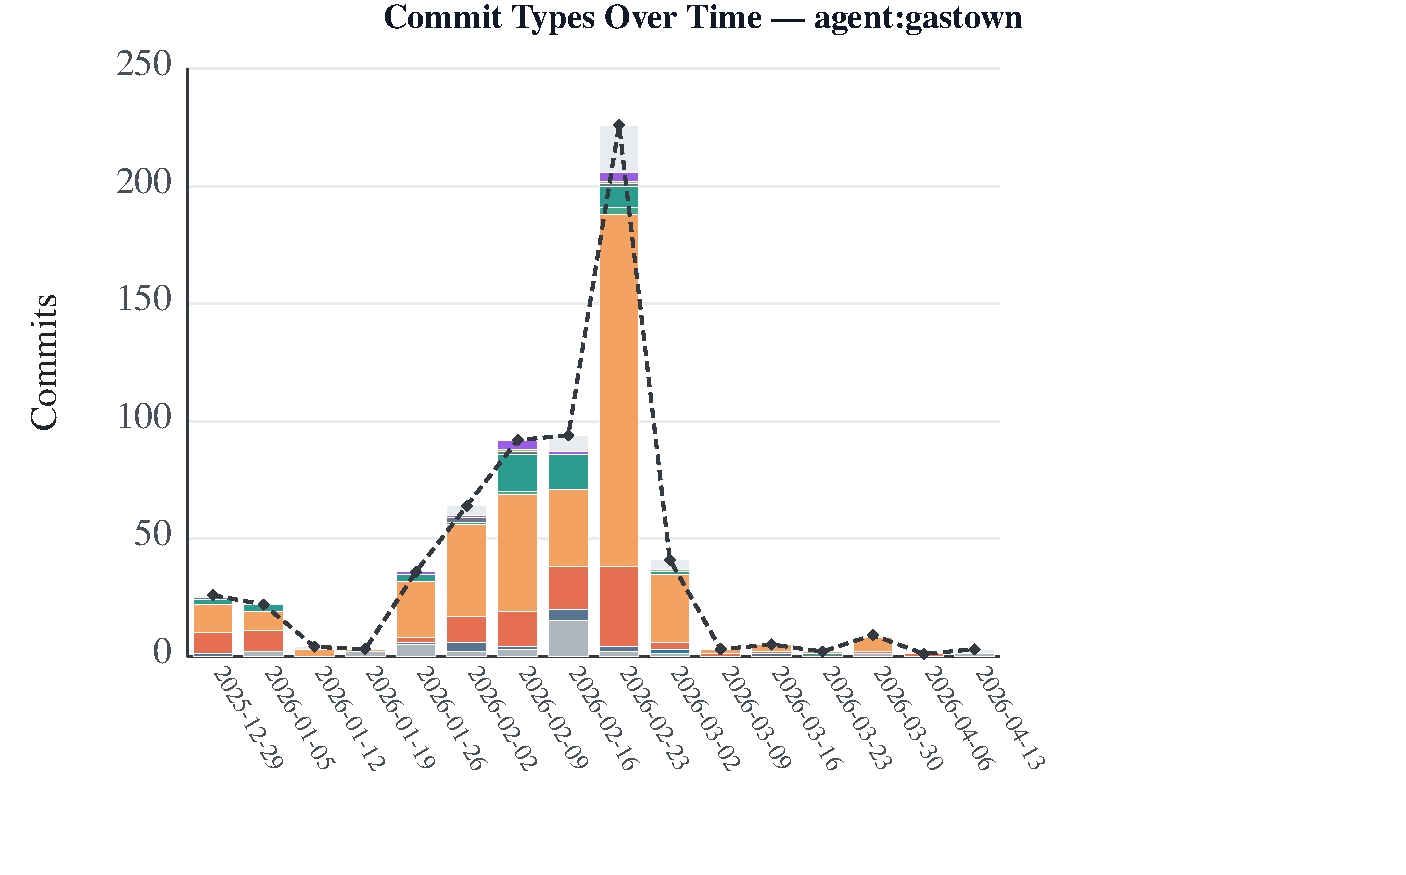
\includegraphics[width=\linewidth]{figures/rq2/commit-types-agent-gastown.pdf}
  \caption{Gastown}
  \label{fig:rq2-gastown}
\end{subfigure}

\begin{subfigure}{0.47\textwidth}
  
\includegraphics[width=\linewidth]{figures/rq2/commit-types-agent-opencode.pdf}
  \caption{OpenCode}
  \label{fig:rq2-opencode}
\end{subfigure}\hfill
\begin{subfigure}{0.47\textwidth}
  
\includegraphics[width=\linewidth]{figures/rq2/commit-types-agent-cursor.pdf}
  \caption{Cursor}
  \label{fig:rq2-cursor}
\end{subfigure}

\begin{subfigure}{0.47\textwidth}
  
\includegraphics[width=\linewidth]{figures/rq2/commit-types-agent-claude_code.pdf}
  \caption{Claude Code}
  \label{fig:rq2-claude_code}
\end{subfigure}\hfill
\begin{subfigure}{0.47\textwidth}
  
\includegraphics[width=\linewidth]{figures/rq2/commit-types-agent-amp.pdf}
  \caption{Amp}
  \label{fig:rq2-amp}
\end{subfigure}
\caption{Distribution of commit types per agent harness. Each chart shows the proportion of conventional commit types (e.g., feat, fix, refactor) for commits attributed to a specific harness.}
\label{fig:rq2-commit-types-per-agent}
\end{figure*}

